
\section{Threat Model and Privacy Objectives}
\label{sec:threat_model}

I define the application context as interactions with mobile devices that involve directing speech toward the device.
 This agrees with typical usage patterns of mobile devices with regards to keyphrase recognition (Figure \ref{fig:keyphrase_application_context}).
 This definition for our application context allows us to leverage difference in the audio signal caused by the directionality of sound waves. 

\begin{figure}[!th]
\centering
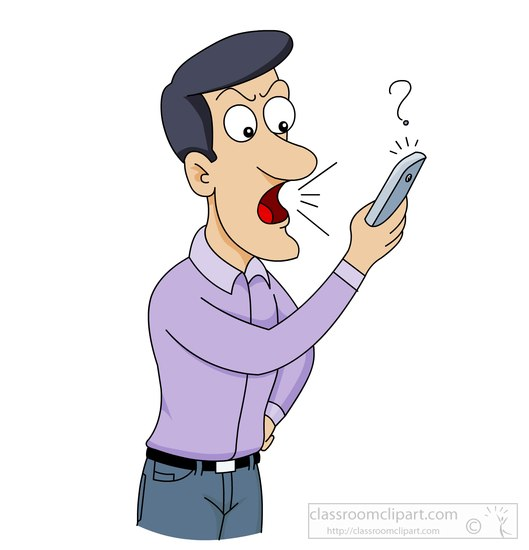
\includegraphics[width=0.4\textwidth]{sound/talking-into-cell-phone.jpg}
\caption{Keyphrase Recognition Application Context}
\label{fig:keyphrase_application_context}
\end{figure}

% \TODO{figure showing the difference in recorded audio when the phone is facing the user/away from the user or in the user's pocket or on the table etc.}

% \TODO{figure showing the difference in recorded audio when the user is speaking into the mic in the headset as opposed to general speech.}


I choose a list of common keyphrases \ref{tab:common_keyphrases} for evaluating the "utility" (keyphrase spotting performance) of my solution.
 The ambient noise in the background while using the application can either be white noise or babble noise.
 I also analyze the effect the intensity of noise has on our keyword spotting performance.

I use the TED-LIUM speech corpus \cite{TEDLIUMCorpus} as a representatitve example of everday conversations in English.
 The corpus also has the advantage of providing English speech examples from speakers with varying accents.
 I also construct babble noise examples by randomly selecting and merging small audio segments from the TED-LIUM speech corpus, as well as borrowing audio snippets from other noise data sets.
 For keyphrase data, I have crowdsourced data acqusition through my Android app and have a rich set of examples for each keyword.
 % \TODO{figure showing number of examples for each keyword and their distribution by male/female, native speaker/non-native speaker, quiet/noisy background}.
 More details on the data acquisition process is described in Section \ref{sec:system_design}.


\begin{table}
\centering
\begin{tabularx}{0.4\textwidth}{| l | l |}
okay google & call mom \\
hey siri & take a picture \\
hey cortana & play a song \\
nine one one & make a note \\
\end{tabularx}
\caption{Common keyphrases chosen for prototyping privacy-preserving algorithms}
\label{tab:common_keyphrases}
\end{table}


\subsection{Rogue Mobile Applications}

The user installs an application "A" on his mobile device to assist with a particular task.
 The application "A" provides a voice interface for everyday use and is granted access to the microphone.
 However, the application "A", however is malicious and records everyday conversations of the user and transmits the audio content to a remote database.
 An attacker uncovers sensitive information from the audio in the remote database using speech recognition.

This is a threat model when applications have access to raw audio data.

\subsection{Adversarial Database Queries}

The user installs an application "A" on his mobile device to assist with a particular task.
 The application "A" provides a voice interface for everyday use and is granted access to obfuscating audio that is sufficient for its voice interface.
 The obfuscated audio data is stored in a database to improve the voice interface of the application.
 An attacker has prior knowledge of a keyword whose presence/absence (binary query) would indicate sensitive information of value.
 The attacker uncovers some sensitive information with a sequence of binary queries using keyword spotting.


This is a threat model when applications have access to obfuscated audio data.


